\documentclass[3p]{elsarticle}

\usepackage{tgpagella}

\usepackage{hyperref}
\hypersetup{
	colorlinks=true,
	linkcolor=blue,
	filecolor=magenta,      
	urlcolor=black,
}
\usepackage[table, dvipsnames]{xcolor}
\usepackage{graphicx}
\usepackage[linesnumbered, ruled, longend]{algorithm2e}
\usepackage{amsmath, amssymb}

%%%%%%%%%%%%%%%%%%%%%%%
%% Elsevier bibliography styles
%%%%%%%%%%%%%%%%%%%%%%%
%% To change the style, put a % in front of the second line of the current style and
%% remove the % from the second line of the style you would like to use.
%%%%%%%%%%%%%%%%%%%%%%%

%% Numbered
%\bibliographystyle{model1-num-names}

%% Numbered without titles
%\bibliographystyle{model1a-num-names}

%% Harvard
%\bibliographystyle{model2-names.bst}\biboptions{authoryear}

%% Vancouver numbered
%\usepackage{numcompress}\bibliographystyle{model3-num-names}

%% Vancouver name/year
%\usepackage{numcompress}\bibliographystyle{model4-names}\biboptions{authoryear}

%% APA style
%\bibliographystyle{model5-names}\biboptions{authoryear}

%% AMA style
%\usepackage{numcompress}\bibliographystyle{model6-num-names}

%% `Elsevier LaTeX' style
\bibliographystyle{elsarticle-num}
%%%%%%%%%%%%%%%%%%%%%%%

%%%%%%%%%%%%%%%%%%%%%%%%
\setlength{\parindent}{10pt}
\setlength{\parskip}{6pt}
%%%%%%%%%%%%%%%%%%%%%%%%
\newtheorem{thr}{Theorem}
\newdefinition{df}{Definition}
\newproof{pf}{Proof}
%%%%%%%%%%%%%%%%%%%%%%%%
\usepackage{color}
\definecolor{light-gray}{gray}{0.95}
%%%%%%%%%%%%%%%%%%%%%%%%
\usepackage{scalerel}
\DeclareMathOperator*{\uint}{\scalerel*{\rotatebox{8}{$\!\scriptstyle\int\!$}}{\int}}

\begin{document}

\begin{frontmatter}

%\title{An efficient approximate algorithm for achieving $(k-\omega)$ angle barrier coverage in camera wireless sensor networks}
\title{An efficient method to verify and assess ($k-\omega$) coverage in wireless multimedia sensor networks}

%% Group authors per affiliation:
%\author[1]{Nguyen Thi My Binh}
%\ead{binhntm@haui.edu.vn}
%\author[2]{Chu Minh Thang}
%\ead{mthang129@gmail.com}
%\author[3]{Huynh Thi Thanh Binh}
%\ead{binhhtt@soict.hust.edu.vn}

\begin{abstract}
Barrier coverage problems in Wireless Camera Sensor Network (WCSN) have attracted increasing interest by academic community because of their huge potential in applications. Almost traditional barrier coverage problems focus on detecting object crossing the barrier sensors. However, only detecting the object may be not sufficient, i.e. when detailed information about the object such as image at a certain view is required. This study aims at analyzing conditions to achieve barrier coverage under a novel multiple view coverage model in WCSN (hereinafter MVBC problem), and then estimating quality of the sensor barrier obtained by devising measure as differentiation field intensity function. The MVBC problem ensures both detecting intruder and recognizing the face of intruder when the intruder comes cross the sensor barrier while requires only a fixed number of sensor nodes. The dynamic partition method is then proposed to solve the MVBC problem. We theoretically show that our differentiation field intensity function is more practical than other existing intensity functions. By conducting intensive experiments, the result indicate that our proposed method provides high quality and stable solutions. The empirical results also show that our new measure provides a good metrics for estimating how well information of an object crossing the barrier can be obtained.
\end{abstract}

\begin{keyword}
minimal exposure path\sep wireless sensor networks\sep stationary sensor networks\sep mobile sensor networks
\end{keyword}

\end{frontmatter}
%\linenumbers
\section{Introduction}
\label{sec:intro}
Barrier coverage in WSNs is a critical issue for various sensor network security applications, e.g., boundary surveillance (national border, critical resource protection) and intrusion detection. Barrier coverage is formed by a sensing barrier for detecting intruders crossing a region of interest. With aiming at monitoring and detecting intruder of sensor networks, barrier coverage requires much less quantity of sensors and energy then full coverage. Thus, barrier coverage is considered more efficient, scalable and attractive in large-scale security applications in reality. Most prior research about the barrier coverage problems aim at building as many as sensor barriers with efficient cost to only detect intruder. In reality, only detecting object is not enough in some scenarios, i.e. there was a terrorist at the airport. In such circumstances, a face recognition system is rather needed. This article investigates a new model of barrier coverage problem in wireless camera sensor networks called MVBC problem as followed: given a WCSN including camera sensor nodes deployed randomly in the interest of region. Under a novel multi-view model coverage which ensures the face of intruder usually to be caught no matter where the directional of face intruder, we verify whether can a barrier of the camera sensor nodes be formed which guarantees both detecting and recognizing unauthorized intruder. We then devise a metric to estimate quality of the achieve barrier. \par
Recently, with multimedia technique development, especially camera sensor networks (CSN) have drawn the attention of research community [1-6]. CSNs can harvest much richer information of the environment in the forms of images or videos than conventional scalar sensors, and thus promise an extremely potential in applications. Thus, security surveillance or intrusion detection application is expected to build up camera sensor barriers efficiently such that every image of intruder can be gathered more details. However, the barrier coverage problem in WCSN generally and the MVBC problem particularly is much different and more complicated than the conventional barrier coverage problem. When sensing range of a chain of camera sensors across the surveillance region is simply combining, that does not provide effective barrier coverage. Because an intruder may cross the barrier without being recognized, i.e., its face image could not be caught. The  fundamental difference between camera and traditional scalar sensors in coverage is that camera sensors may capture very different scenes of the same object if they are from different viewpoints. For instance, when a camera is placed behind the intruder, no face image can be recognized. In the computer vision field, researches show that the object is more likely to be recognized by the recognition system if the image is captured at or near the frontal viewpoint \cite{blanz2005face}, i.e., if the object is facing straight to the camera. As the angle between the object facing direction and the camera viewing direction increases, the detection rate decreases dramatically. Therefore, to keep a high level monitor quality, a good camera sensor barrier should ensure that no matter where the traversing object faces, there is always some camera to effectively capture its face image.\par
%
To obtain more information of the stable objects, especially their face identifications, full-view coverage model was first introduced by Wang and Cao [8, 9]. An object is full-view covered if there is always at least one camera covering it no matter which object facing direction and the cameras viewing direction is sufficiently close to the object facing direction. Obviously, we can obtain more information about the intruder in full-view model. In \cite{wu2012achieving}, the authors provide the necessary and sufficient conditions to achieve full view coverage under uniform deployment and Poisson deployment. \par
%
Ma et al. \cite{ma2012minimum} studied the minimum camera barrier coverage problem in WCSNs when the camera sensors are deployed randomly in a monitor field. The authors have some extension, the algorithm reduces the number of camera sensors, but it still requires a lot of camera sensors to construct a full viewed barrier coverage. In \cite{xu2016minimum}, Xu et. al. also want to maintain the quality of aggregate information with the least camera sensors. Basing on $(k-\omega)$ angle coverage model \cite{tseng2012k}, they produce a new barrier coverage model named by $(k, \omega)$-angle barrier coverage. The object is said $(k-\omega)$ angle coverage when it is simultaneously monitored by at least k sensors, and to ensure that k different sensors monitor different parts of the object, the angle between two arbitrary sensor directions must be equal or greater. The monitored field exists a $(k-\omega)$ angle barrier coverage if it has a connected region across the monitor field such that every point within the region is $(k-\omega)$ angle coverage. The $(k-\omega)$ angle barrier coverage is useful because of a balance of the number of camera sensors used and the information retrieved by the camera sensors.\par
%
However, a fundamental problem of assessing the quality of a $(k-\omega)$ angle barrier has not been addressed. Currently, in the tradition model of attenuation, when evaluating the coverage quality of a sensor toward a certain point, the coverage value formula is defined to be affected only by the distance from the sensor to the considered point, which may lead to several exceptional inconsistency regarding evaluate the quality of coverage, especially in the problem of $(k-\omega)$ barrier in the sensor network. Firstly, the model can only illustrate the general coverage of a point to a certain sensor. As a result, it is impossible to achieve a metric measuring the amount of information on every direction of an intruder captured by the network of sensors, which is fundamental in several coverage problems such as the $k-\omega$ cover or the full view cover problem. Secondly, this model shows little consistency considering the coverage of a point in a sensor network. In case of evaluating the coverage of a point exposed to numerous sensors, there have been 2 common models, the All-Sensor Field Intensity and the Closest-Sensor Field Intensity model. While the latter failed to illustrate the cooperation of the sensors in sensing the same object, which greatly underrate the real coverage of the network on the intruder, the former model does not take into account the repetition of information captured by numerous sensors, thus exaggerate the value of coverage dramatically.\par
%
As a result, we found it necessary to devise a more preferable attenuated model assessing the coverage quality of the sensor network toward a point in the field of interest, the model can later be generalised to evaluate the coverage of the sensor network on a line or a closed region. To formulate the coverage value regarding information from every direction of the intruder, it is necessary to consider its shape. In this article, the problem is tackled generally, which results in we using the rule of symmetric to make an assumption that the intruder is a circle. This geometrical shape is sufficient since the coverage is considered in the 2-D plane only, and the circle itself has parts of the circumference followed every possible direction, which help illustrate the devised model more thoroughly and clearly.\par
%
The coverage model implements the idea of Divide-And-Conquer. The intruder is differentiated into several small parts. Each of them is then evaluated separately, then added together to obtain the total coverage of the sensor network on the intruder at the considered position. Each small part of the circle, in turn, is calculated with each sensor that cover it, then the largest coverage value is taken. This operation will prevent the coverage overrated from several sensors having similar position toward the considered point, which in real life will serve no purpose of obtaining more information of the specific part on the intruder. 

Camera sensors are randomly scattered for achieving barrier coverage in a large scale which is a very challenged.\par
%
In this paper, we focus on evaluating a sensing field based on two factors: the probability of successfully forming a $(k-\omega)$ angle barrier, and the average quality of the found barriers in the sensing fields. This problem is vital for optimizing the efficiency of sensor placement in sensor networks when camera sensor nodes were deployed randomly. For instance, camera sensors have to be scattered by plane or artillery if the region of interest is hostile or inaccessible or deficiency on time, manpower or funds prevents careful arrangement of every single sensor.\par
%
The main contributions of this article are as follows. 
\begin{itemize}
	\item Formulate achieving ($k-\omega$) angle barrier coverage problem.
	\item Propose an efficient method to deterministically verify if a monitored field can be achieved a ($k-\omega$) angle barrier coverage in by any given set of camera sensors. 
	\item Evaluate the found barriers with the devised metric.
	\item Conduce experiments in various scenarios to examine the result and the computation time of the proposed algorithm.
	\item Analyze and estimate the parameters effect on performance of proposed algorithm.
\end{itemize}
%
The rest of the paper is organized as follow. Related works are presented in section 2. Section 3 formulates A ($k-\omega$) angle barrier problem. Section 4 introduces proposed algorithm. Section 5 gives our experiments along with computational and comparative results as well as conclusion in section 6.
%

\section{Related works}
The concept of barrier coverage \cite{kumar2005barrier}, was first introduced specifically for intruder detection applications in WSNs where sensing regions of sensor nodes form one or multiple barriers so that any intruder penetrating the region of interest will be detected. Due to its superiorities for security applications, barrier coverage has received attentions in recent years. The barrier coverage problems in WSNs can be categorized into two sub-problems: one is finding penetration paths. A penetration path is continuous curve with arbitrary shape, spanning from one side to the other side of a sensor field; other is building intrusion barrier for detecting intrusion of a mobile object when it traverse from on side to the other side of the sensing field. The formal problems have thoroughly been delved into many researches such as \cite{megerian2002exposure,binh2016heuristic,liu2013percolation,binh2017genetic,binh2019efficient}, the latter ones mostly focused on critical condition analysis (e.g., sensor node density) and barrier construction for stationary sensors with omni-directional sensing coverage models. \cite{liu2008strong,saipulla2008barrier,he2010distributed,skraba2007energy,chen2013energy}. Directional sensing coverage models then were widely used such as camera, radar etc., and taken into consideration in coverage problems as well as in barrier coverage problems.
 \cite{ai2006coverage,akyildiz2007survey,guvensan2011coverage,ma2005coverage,soro2005coverage}. Barrier coverage problems in WCSNs are much more complexed and challenging compared to those in traditional scalar WSNs \cite{chang2006collaborative,ma2012minimum,makhoul2009adaptive,wang2011barrier}, because of WCSNs having unique features.
 
 The authors \cite{chang2006collaborative} proposed a collaborative technique for face
 analysis in WCSNs with a dual objective of
 detecting the camera view closest to a frontal view of the
 object, and assessing angles between the face directional and all the camera views based on additional fusion of local angle estimates. To gather more information of the stable object, especially face recognition, full-view coverage was introduced in \cite{wang2013achieving} by Wang et al. An object is full-view covered if its face is always a camera to cover it no matter which face direction and the angle between the camera’s viewing direction and the object’s facing direction is less than a predefined parameter $\theta$. The authors proposed a method for full-view coverage verification on a sensing field. After that, they derived an estimation of the sensor density needed for full-view coverage in a random deployment. Based on this work, Wang et al. further studied the problem of constructing a camera barrier in \cite{wang2011barrier}. They proposed a method to select camera sensors from an arbitrary deployment to form a camera barrier and then presented a technique for reducing the number of cameras used since there might be redundant cameras (cameras that can be turned off without breaking the barrier) after barrier is formed.
 Besides, Ma et al. \cite{ma2012minimum}, proposed a better method for constructing camera barrier. With aiming at minimum the number of camera sensors in full-view barrier coverage, the problem is transformed into the shortest path problem from the source to the destination node on graph. \textcolor{ProcessBlue}{\bfseries However, the algorithm using in this work cannot be used to solve the problem}. This algorithm can be considered as a variant of Dijkstra algorithm. The only two differences are: (1) the edge has no weight but each vertex $v$ has a "weight" denoted by $I(v)$ and (2) the operator used for updating label of a vertex is union instead of addition. The second difference is the reason why the algorithm has problem. According to the algorithm, when a vertex $v$ is labeled, every previous vertex in the path from source vertex $s$ to $v$ is also labeled. Supposed $u$ is such a vertex between $s$ and $v$, the shortest path from $s$ to $u$ must be contained in the path from $s$ to $v$. But this is not true when the operator union is used, Figure \ref{fig:01} illustrates this.
 
\begin{figure}[p]
	\centering
	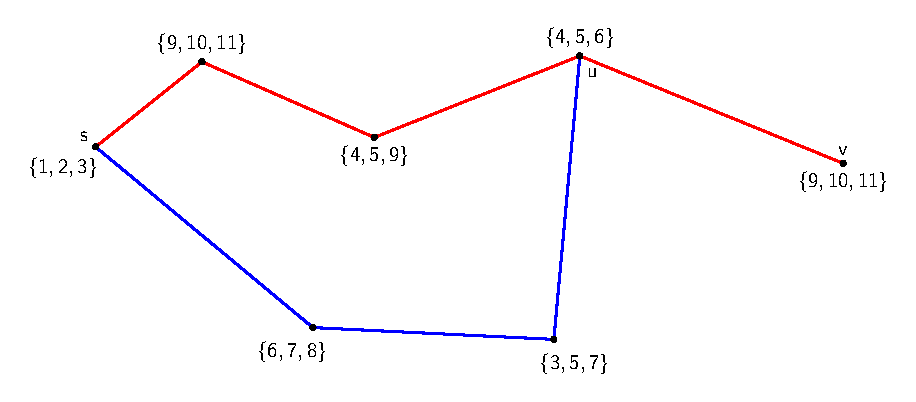
\includegraphics[scale=0.6]{wrongDijstra.pdf}
	\caption{Red line is shortest path from $s$ to $v$. Blue line is shortest path from $s$ to $u$}
	\label{fig:01}
\end{figure}

To monitor the object from multiple perspectives, Tseng et al. \cite{tseng2012k} introduced the notion of $k$-angle coverage. To avoid duplicating information from multiple sensors simultaneously monitoring an object, an angle constraint was added, which guaranteed  any two sensors cannot appear in an angle range of $\omega$ around the object (Figure \ref{fig:02}). It was pointed out that if an object is $(k-\omega)$ angle covered, there is no angle larger than $2\pi-(k-1)\omega$ of the object that is not covered by any sensor. This means that an object that is $(k-\omega)$ angle covered is also full-view covered with parameter $\theta=\displaystyle\frac{2\pi-(k-1)\omega}{2}$. Hence, $(k-\omega)$ angle coverage can be considered as a special case of full-view coverage with the number of camera sensors covering the object is fixed. Under this new coverage model, the paper focused on maximizing number of static objects that are covered using minimum number of sensors.
\begin{figure}[p]
	\centering
	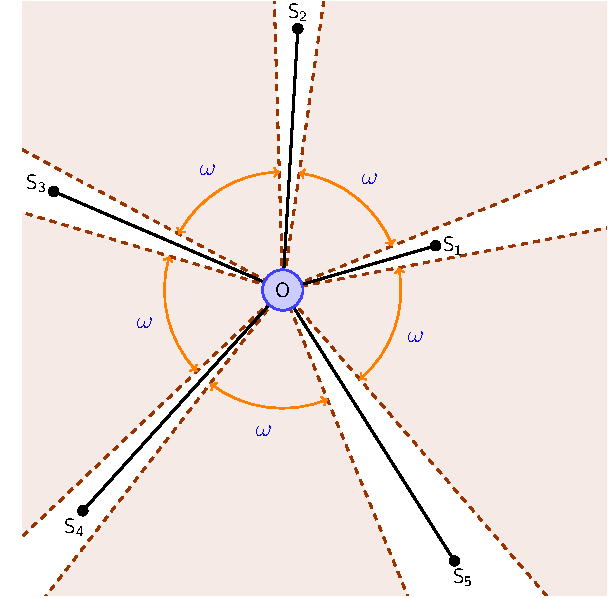
\includegraphics[scale=0.6]{komega.pdf}
	\caption{$O$ is 5-$\omega$-angle covered by $\{S_1, S_2, S_3, S_4, S_5\}$}
	\label{fig:02}
\end{figure}

In \cite{xu2016minimum}, the authors studied the problem of constructing $(k-\omega)$-angle barrier using minimum number of sensors called MkABC. The paper presented MkABC problem in two sensor deployment schemes. Under deterministic deployment, a geometric method was proposed, which used the feature of regular polygon to construct a ($k-\displaystyle\frac{\pi}{k}$)-angle barrier. When sensors are randomly deployed in the ROI, the MkABC becomes more difficult. In this scenario, the authors proposed a grid-based method, where each grid is judged to be $(k-\omega)$-angle covered or not. MkABC problem is then transformed into the shortest path problem on graph. The algorithm used is the same as one used in \cite{ma2012minimum}, which has some problems as aforementioned. Besides, The grid-based method has a trade-off between solution accuracy and the computational cost, which all depend on grid size chosen. This is a big disadvantage of this approach in large-scale WSN. 

Chen et al. \cite{chen2008measuring} first mentioned the problem of measuring the quality of barrier coverage in ODSNs. According to that, just consider whether or not a sensor network providing barrier coverage, which is equivalent to measuring its quality as either 0 or 1, is not enough since there might be many different levels of quality coverage of the sensor barrier. The authors introduced the notion of $L$-local $k$-barrier coverage to measure the quality of $k$-barrier coverage for a belt region as the maximum value of $L$ that the belt is $L$-local $k$-barrier covered. A belt region is said to be $L$-local $k$-barrier covered if every zone of length $L$ in the region is $k$-barrier covered. Two other metrics that they had considered are: (1) the number of sensors needed to make the belt k-barrier covered and (2) the probability that an intruder following a randomly picked path being detected by at least k sensors. All these metrics can effectively measure the coverage quality, however, they always provide the same result when sensor network has already achieved k-barrier coverage, i.e, the probability of detecting the intruder by $k$ sensors is always 100\%. In addition, the considered k-barrier is just combination of consecutive sensing range. Actually, these metrics reflect constructing level of k-barrier, i.e. the closer distance L and the length of the strip region is, the more ROI achieves k-barrier. In contrast, our purpose evaluates quality of collected information in camera sensor barriers. This prompts us to devise a novel metrics called Differential coverage.  

%After considering many related works, we see that previous researches about barrier coverage problems in WCSNs are not yet efficient and there are rooms for improvement. Basing on $(k-\omega)$-angle coverage model \cite{xu2016minimum} with some fine-tuned for adapting to monitor mobile objects in barrier coverage in WCSNs, which refers to multiple view coverage model. Therefore, we produce the multiple view barrier coverage problem in WCSNs, then propose method as \textcolor{ProcessBlue}{\bfseries Dynamic Partition} to solve this problem. Furthermore, we desire to measure the quality of object's information recorded by sensors network when it crosses the barrier. Since the metrics proposed in \cite{chen2008measuring} is for $k$-barrier coverage model in ODSNs, it cannot apply to our problem. Moreover, this metrics only works when sensors network has not provided $k$-barrier coverage yet. In contrast, we need a metrics for measuring quality coverage of the barrier, which means the barrier must have been already constructed. These have fostered us to devise a new metrics called \textcolor{ProcessBlue}{\bfseries Differentiation Exposure}.




\section{Preliminaries and problem formulation}
\subsection{Preliminaries}

%{\bfseries Definition 1: } {\itshape$(k-\omega)$ coverage}
%\subsubsection{($k-\omega$) region of a k-sensor list}
\begin{df} 
{\itshape$(k-\omega)$ coverage}
\begin{itemize}
	\item A point $P$ is said to be $(k-\omega)$ covered if there exists a list of $k$ sensors $L = \{S_1, S_2,...,S_k\}$ ordered in counter-clockwise order around $P$, such that $\omega < (\overrightarrow{PS_i}, \overrightarrow{PS_{i+1}}) < \pi, \forall i \in \{1,2,...,k\}$.
	\item A region $R$ is said to be $(k-\omega)$ covered if every point in $R$ is $(k-\omega)$ covered.
\end{itemize}
\end{df}
\begin{df}
{\itshape Inner safe region of a polygon's side.}\par
Given a polygon {\sc pol}. Let $AB$ is a side of {\sc pol}. The way to determine the inner safe region is as follows:
%\vspace{-5pt}
\begin{itemize}
	\item Choose the midpoint $M$ of $AB$.
	\item Draw an arrow from $M$ toward the inner region of {\sc pol}.
	\item The safe region of $AB$ consists 2 symmetrical parts splitted by line $AB$. The part that the arrow points to is the inner safe region of $AB$.
\end{itemize}
\end{df}
Figure ~\ref{innersafe} is an illustration of inner safe region of $S_1S_2$.
\begin{figure}[!h]
	\begin{center}
	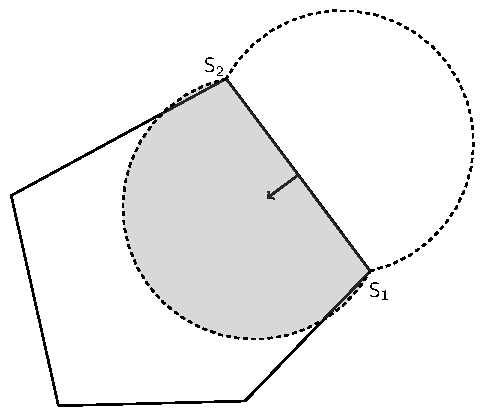
\includegraphics[scale=1.]{innersafe.pdf}	
	\caption{inner safe region of $S_1S_2$}
	\label{innersafe}
	\end{center}
\end{figure}
\begin{df}
{\itshape($k-\omega$) region of an $k$-sensor ordered list}\\
Given a $k$-sensor ordered list $L = \{S_1,S_2,...,S_k\}$. ($k-\omega$) region of $L$ is the locus of points that are ($k-\omega$) covered by $L$.
\end{df}
\begin{thr}
{\itshape($k-\omega$) region of an $k$-sensor ordered list $L =\{S_1,S_2,...,S_k\}$ is the intersection of inner safe region of every line segment $S_iS_{i+1}$ and the sensing range of all sensors in $L$}.
\end{thr}
\begin{pf}
	Let $R$ denote the ($k-\omega$) region of $L$. We only consider the case that $R$ is not empty. Suppose that $P$ is a point inside $R$, then $P$ is ($k-\omega$) covered by $L$. From definition 1, we have $(\overrightarrow{PS_i}, \overrightarrow{PS_{i+1}}) > \omega$ (1) and $(\overrightarrow{PS_i}, \overrightarrow{PS_{i+1}}) < \pi$ (2),\ $\forall i \in \{1,2,...,k\}$. Condition (1) means that $P$ is inside the safe region of $S_iS_{i+1}$. This safe region has 2 symmetrical parts splitted by line $S_iS_{i+1}$. Condition (2) forces $P$ to be located at only one special part which satisfies $(\overrightarrow{PS_i}, \overrightarrow{PS_{i+1}}) < \pi$. And this part is always the inner safe region of $S_iS_{i+1}$. Hence, $P$ is inside the intersection of inner safe region of every line segment $S_iS_{i+1},\ i=\overline{1,k}$ and the sensing region of all sensors in $L$ (call this intersection $\mho$) (*).\par
\indent On the other hand, if $P$ is inside $\mho$, $P$ satisfies the condition (1) and (2). Thus, $P$ is ($k-\omega$) covered by $L$, which deduce to $P$ is inside $R$ (**).\par
\indent From (*) and (**), we have theorem 1 proved.
\end{pf}
\begin{thr}
{\itshape($k-\omega$) region of an $k$-sensor ordered list $L =\{S_1,S_2,...,S_k\}$ is a convex region}.
\end{thr}
\begin{pf}
The intersection of two convex regions is a convex region. Hence, the intersection of any limited sets of convex region is a convex region. From theorem 1, it is obviously that ($k-\omega$) region of a list $L$ is intersections of convex regions and thus, we have theorem 2 proved.
\end{pf}
Figure 2 is an illustration of this theorem. By that, the blue hatching area is the ($k-\omega$) region of $L=\{S_1,S_2,S_3,S_4\}$ and $\omega = 60$.
\begin{figure}[h]
\begin{minipage}{.5\linewidth}
	\centering
	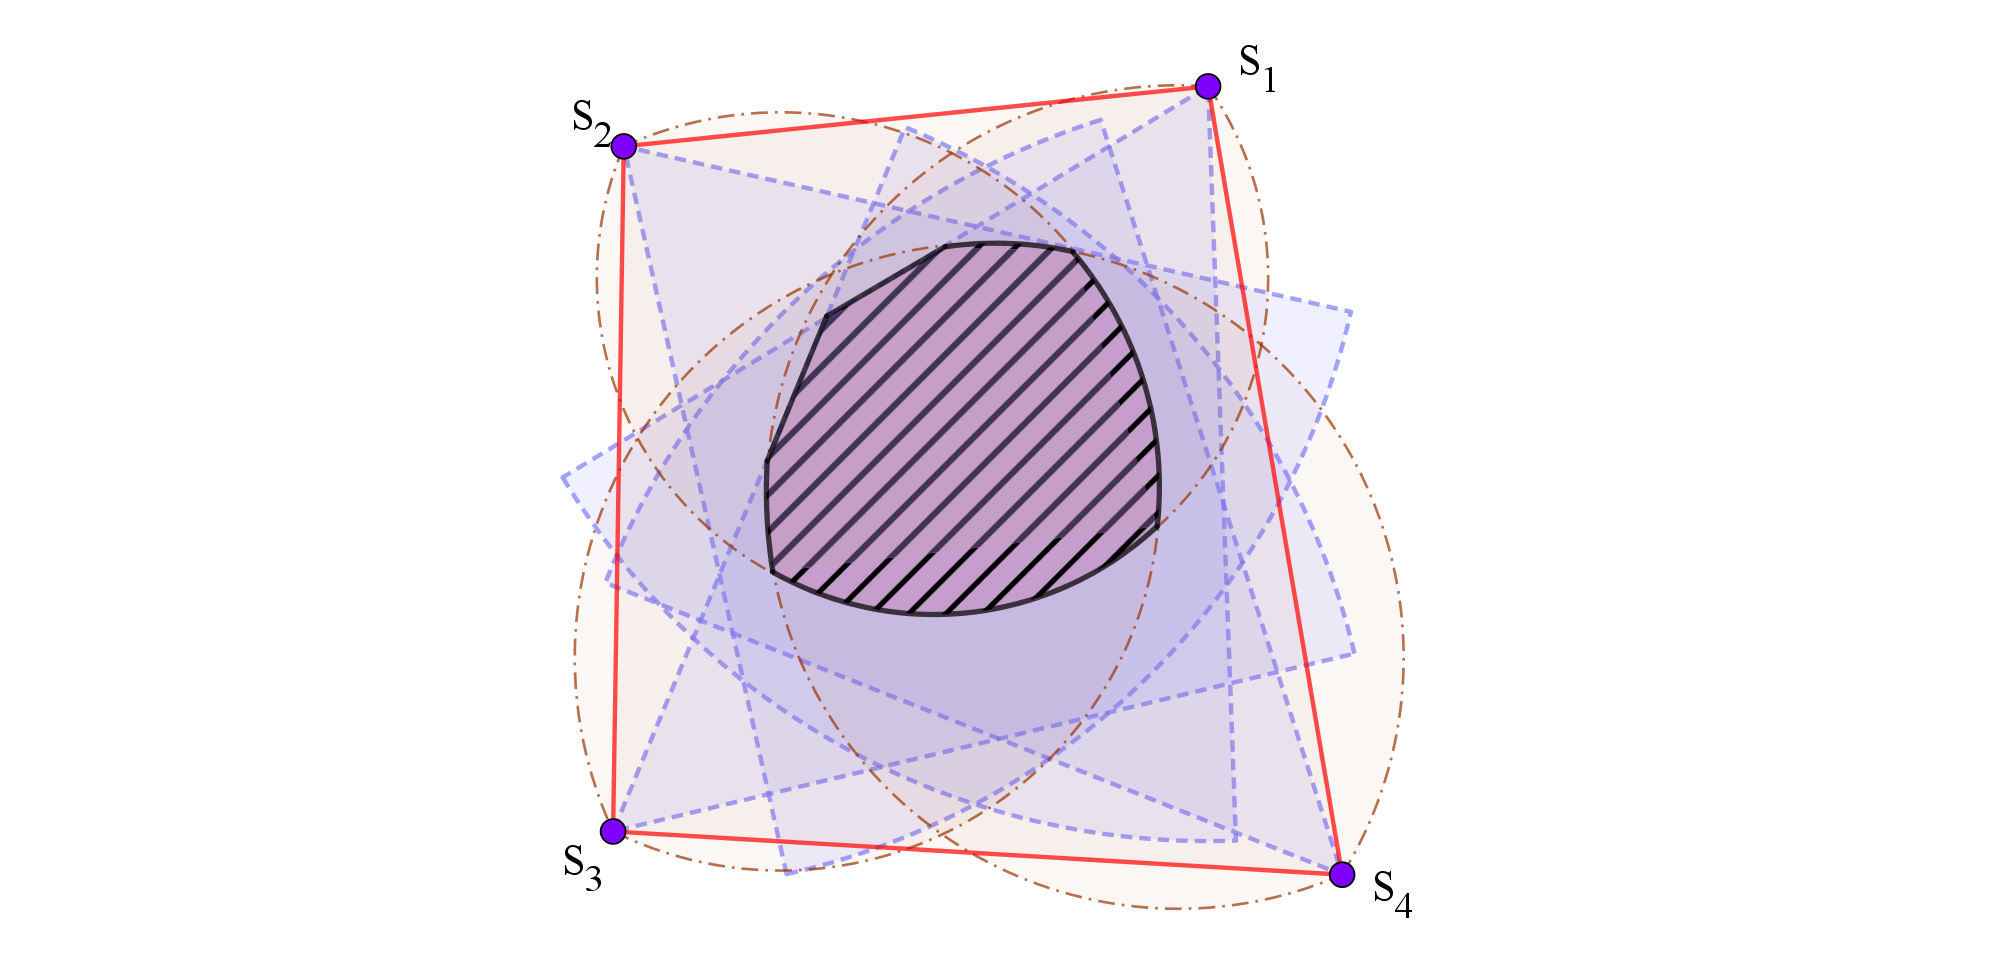
\includegraphics[scale=0.9]{hinhminhhoa.png}
\end{minipage}
\caption{($k-\omega$) region of $L=\{S_1,S_2,S_3,S_4\}$ and $\omega = 60$}
\end{figure}

We provide some preliminaries used in the following sections of this paper.
\begin{df}
	{\itshape Differentiation Field Intensity}
\end{df}
In the tradition models to evaluate the coverage from the sensing field toward the point may lead to several exceptional inconsistency due of these model just depend on distance between sensors in sensing field and the considering point. As a result, we devise a more preferable attenuated model assessing the coverage quality of the sensor network toward a point in the field of interest, the model can later be generalized to evaluate the coverage of the sensor network on a line or a closed region.

Considering a point lie in the sensing range of a certain omnidirectional or directional sensor. The sensor $S_i$, the penetration object $P$ with radius $R$ and the considered part $P_\phi$ being positioned at $\phi$ and has length $dl$. Call the distance from $S_i$ to $P_\phi$ as $d_i$, the direction of the sensor compared to the pivot direction as $\phi_i$. Because $R$ is usually inconsiderable compared to $d_i$, we can approximately use $\phi_i$ and $d_i$ as constants with variable $\phi$, the model will be now illustrated as followed.

\begin{figure}[h]
\begin{minipage}{.5\linewidth}
	\centering
	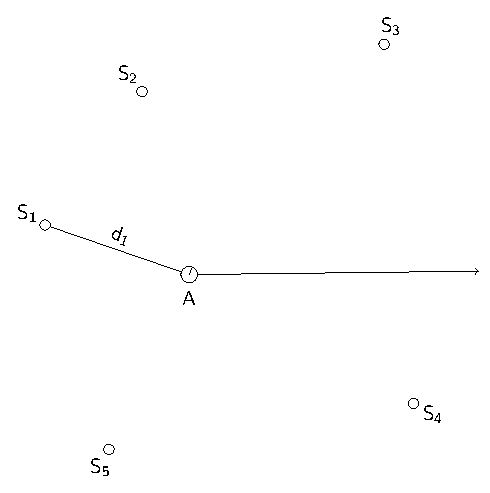
\includegraphics[scale=.75]{groupSensor_Version2.pdf}
\end{minipage}\hfill
\begin{minipage}{.5\linewidth}
	\centering
	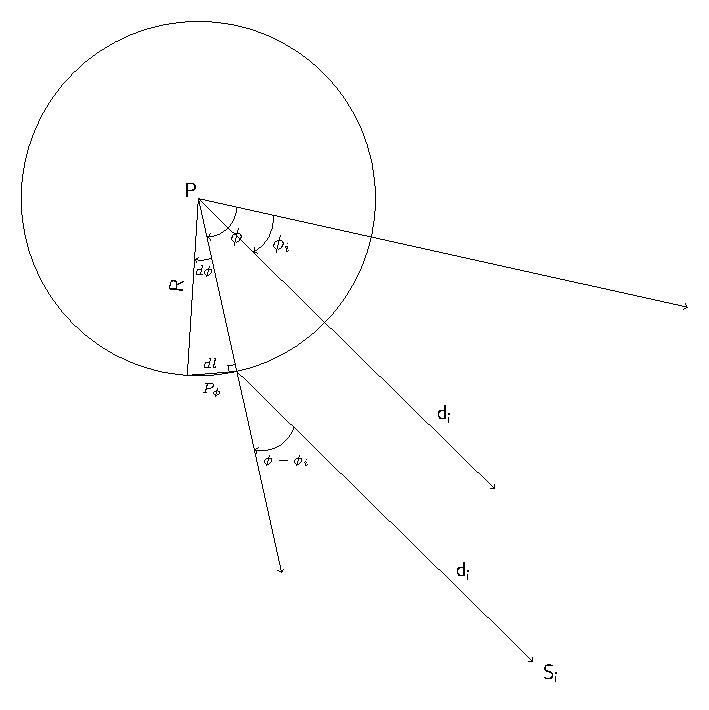
\includegraphics[scale=.6]{exposure.pdf}
\end{minipage}
\end{figure}

Firstly, the coverage value of a sensor to a part is directly affected by the distance between the sensor and the part, and the angle at which the part is viewed by the sensor, this results in the formula:
\begin{equation}
\label{eq1}
\mathsf{max}(\frac{A\cos(\phi - \phi_i)}{Rd_i^\lambda}, 0)dl
\end{equation}


where $\frac{A}{R}$ is a constant coefficient, note that the coverage would fall below 0 if the angle between the direction of the part and the direction of the sensor is larger than $\frac{\pi}{2}$, so we need to set it to 0 in that case. Rewrite $dl = Rd\phi$, we have:
\begin{equation}
\label{eq2}
\mathsf{max}\left\{\frac{A\cos(\phi - \phi_i)}{d_i^\lambda},\ 0\right\}d\phi
\end{equation}

However, it is obviously unnecessary to obtain too much detailed information from the object in the sensing field. This leads to the existence of a constant $E_{\mathsf{max}}$ which corresponds to the maximum necessary coverage on a part with unit length of the circle. To isolate the value from the relative constant $A$, we rewrite it to the Minimum sensing radius $E_{\mathsf{max}} = \frac{A}{d_{\mathsf{min}}^\lambda}$. As a result, our coverage formula could be rewritten as:
\begin{equation}
\label{eq3}
\mathsf{max}\left\{0,\ \mathsf{min}\Big\{\frac{A}{d_{\mathsf{min}}^\lambda}, \frac{Acos(\phi - \phi_1)}{d_i^\lambda}\Big\}\right\}d\phi
\end{equation}

As a result, the coverage on a part $P_\phi$ of several sensors $S_i$, as illustrated above, is the maximum of the coverage on that part of every covered sensor:

\begin{equation}
\label{eq4}
E_\phi(P) = \mathsf{max}\left\{0,\ \mathsf{min}\Big\{\frac{A}{d_{\mathsf{min}}^\lambda},\ \underset{S_i}{\mathsf{max}}\big\{\frac{A\cos(\phi - \phi_i)}{d_i^\lambda}\big\}\Big\}\right\}d\phi
\end{equation}


In short, the coverage on a part of a certain set of sensors is calculated from the largest value of $\displaystyle\frac{Acos(\phi - \phi_1)}{d_i^\lambda}d\phi$ across all sensors, the result then will be a value in the close interval $[0, E_{\mathsf{max}}d\phi]$ that closest to the above computed value. The total coverage on the object is the sum of the coverage on its small parts. Combined with the differentiated form of the formula above, the total coverage would be the integral on all of its parts. As a result, we receive the formula for the total coverage on the object at a certain point in the sensing field:
\begin{equation}
E(P) = \uint\limits_0^{2\pi}{\mathsf{max}\left\{0,\ \mathsf{min}\Big\{\frac{A}{d_{\mathsf{min}}^\lambda}, \ \underset{S_i}{\mathsf{max}}\big(\frac{A\cos(\phi - \phi_i)}{d_i^\lambda}\big)\Big\}\right\}d\phi}
\end{equation}
In conclusion, a new model of coverage is devised which may prove to be exceptionally effective in measuring the coverage efficiency of sensor networks in not only the tradition coverage problem but also in more complex ones such as the problem of $full\hspace{1mm}view$ or multiple view barrier coverage. The new model is proposed with detailed and precise logical progress, successfully adapts the strong points of both the All-Sensor Field Intensity and the Closest-Sensor Field Intensity model \cite{megerian2002exposure}, handling preferably the cooperation of multiple sensors in the network without overrating the repetition of captured information.
%\subsubsection{Coverage of a barrier}	
%\label{bar	rier}

\begin{df}{\itshape($k-\omega$) barrier}\\
	A ($k-\omega$) barrier $B$ is a connected region from the left side to the right side of the monitoring region and satisfies that $B$ is ($k-\omega$) covered.
\end{df}
\begin{df}{\itshape($k-\omega$) barrier coverage}\\
	A region achieves ($k-\omega$) barrier coverage if there exists a ($k-\omega$) barrier in that region.\par
\end{df}

A $(k-\omega)$ barrier (a multiple view barrier) is a region connects the left and right side of the sensing field in which all the points are $(k-\omega)$ covered. Typically, a multiple view barrier is fairly narrow, and penetration objects usually intersect the barrier only at a small part on their paths. As a result, a proper metric to assess the efficiency of the multiple view barrier would be the coverage density of it.

With the same set of sensors considered, in the range of coverage of all elements of that set, the coverage function is always continuous. Since a barrier is consisted of several separated parts each of which is $k-\omega$ covered by a common set of sensors, the coverage density of the barrier can be defined as the quotient of the total coverage in the barrier and the area of that area, with the total coverage being formulated as the integral of the coverage function over the barrier region. Call the barrier region $B$ with area $S_B$, the coverage density over $B$, which is $D_B$ can be formulated as
\begin{equation}
\label{eq5}
E(B) = \iint_B{E(x, y)dxdy}.\frac{1}{S_B}
\end{equation}


\subsection{Problem formulation}
\subsubsection{Verify the ($k-\omega$) barrier coverage}
The problem is formulated as follows. Given a set of $n$ sensors $S=\{S_1,S_2,...,S_n\}$ and a rectangular region $\Omega$ with the length of $L$ and the width of $W$. $\Omega$ is called the monitoring region and camera sensors in $S$ are deployed according to uniform deployment scheme in $\Omega$ to serve the purpose of observation. The uniform deployment scheme means that total $ n $ sensors are deployed randomly, uniformly and independently.\par

The objective of the problem is to verify if $\Omega$ achieves multiple-view barrier coverage. In other words, we need to determine if there exists a multiple-view barrier $B$ in $\Omega$. If there is none, $\Omega$ will not guarantee security requirements and the sensors need to be re-deployed.\par

Unlike omni-directional sensor, which only provides information about detection of the object, camera sensor is typically directional sensor and can be used to obtain multimedia information of the object. Each camera sensor can be denoted by a 4-tuple $\{S_i, R, \alpha, \varphi_i\}$, where $S_i$ is the location of sensor $i$, $R$ is the sensing radius and $\alpha$ is half of the sensing angle. We assume that all sensors have the same sensing radius and sensing angle. In reality, sensing range of camera sensor is usually less than $\pi$, so we also have an assumption that $\alpha < \displaystyle\frac{\pi}{2}$. The last parameter of a camera sensor, $\varphi_i$, is the facing direction of sensor $i$, which is uniformly distributed in $[0,2\pi]$ \par
Figure \ref{sensing-model} shows information of sensor $s$.
\begin{figure}[!h]
	\centering
	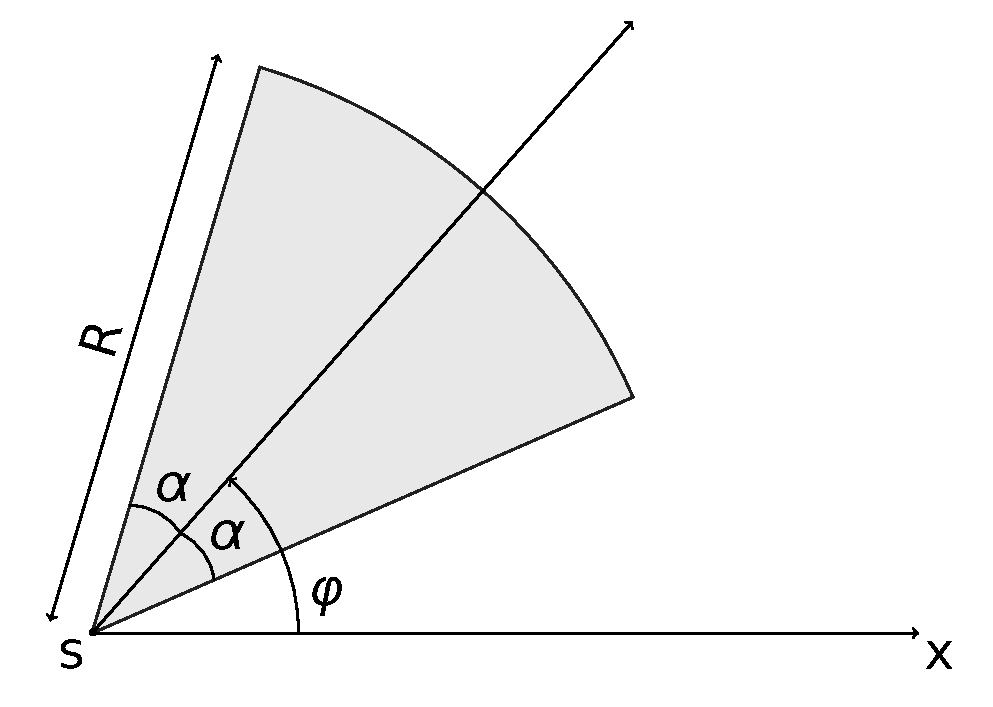
\includegraphics[scale=.5]{Hinhanh/sensing-model2}
	\caption{Illustration of a camera sensor $s$. The shadow area is the sensing region of $s$}
	\label{sensing-model}
\end{figure}

\noindent The input and output of the problem are followings:\\[7pt]
{\bfseries Input}
\begin{itemize}
	\item $L, W$: Length and width of the monitoring region $\Omega$ respectively.
	\item $n$: Number of camera sensors.
	\item $S = \{S_1,S_2,...,S_n\}$: Set of camera sensors. $S_i$ denotes the $i$-th camera sensor and also denotes the location of that sensor.
	\item $R$: Radius of camera sensors.
	\item $\alpha$: Half of the sensing angle of camera sensors.
	\item $\varphi_i$: Orientation angle view of $S_i$ where $i=\overline{1,n}$.
	\item $k, \omega$ : The conditional parameter of the problem.
\end{itemize}
{\bfseries Output}
\begin{itemize}
	\item The yes/no answer that the monitoring region achieves multiple-view barrier coverage. 
\end{itemize}

\subsubsection{Evaluate the quality of a multiple-view barrier}
The problem is formulated as follows. Given a barrier $B$ in a sensing field containing several connected regions $B_i$ from the left to the right boundary of the field. Each $B_i$ is a closing field that is ($k-\omega$) covered by a $k$-list of sensors $P_i$.

The objective of the problem is to find the coverage of the barrier regarding our devised metric. The process is to assess the quality of the found barrier and compare the result with other settings of parameters to analyze the effect of each parameter to the quality of the sensing field and find the best combination of settings to achieve our desire.

\noindent The input and output of the problem are followings:\\[7pt]
{\bfseries Input}
\begin{itemize}
	\item $\{B_i\}$: The set of closing region connect the left and the right edge of the sensing field.
	\item $\{P_i\}$: The set of $k$-list of sensors, the $P_i$ is known to ($k,\omega$) cover the region $B_i$.
\end{itemize}
{\bfseries Output}
\begin{itemize}
	\item The coverage value of the ($k,\omega$) barrier.
\end{itemize}

\section{Proposed algorithm}
\subsection{Verify the ($k-\omega$) barrier cover}
To solve this problem, the monitoring region is partitioned into several small rectangles using the proposed Dynamic Partition method. After that, we try to figure out if there is a continuous barrier from the left side to the right side of the region consisting of rectangles which are multiple-view covered. The details are shown in the subsequent sections.

\subsubsection{multiple-view verification on a rectangle}
\label{subsec:01}
% introduction idea
Based on theorem 2, we can conclude that in order to verify the multiple-view coverage on a rectangle, it is sufficient to check whether all four vertices of that rectangle is multiple-view covered by an common list of sensors. Using this conclusion, we propose an algorithm to verify multiple-view coverage on a rectangle, and for the optimization of the second problem, we try to find the list that multiple-view cover the rectangle with the largest coverage value. 
% 4 steps
%The idea of our algorithm can be described as follows:
The following steps describes the idea to verify if rectangle $ABCD$ is ($k,\omega$) covered:
\begin{description}
	\item[Step 1:] Find a set of sensors $G$ that cover four vertices of the rectangle $ ABCD $.
	\item[Step 2:] Find all lists of $k$ sensors from $G$ satisfies that the point $A$ is ($k,\omega$) covered by these $k$ sensors.
	\item[Step 3:] Among found lists, filter out those which do not simultaneously ($k,\omega$) cover three points $B$, $C$, $D$. This step will offer all lists of sensors that $(k,\omega)$ cover the rectangle $ABCD$. If there does not exist such a list, $ABCD$ is not ($k,\omega$) covered. Otherwise, go to {\bfseries Step 4}.
%	\item[Step 4:] There are 2 possible approaches to choose a single list of sensors in the list of sensor lists found in step 3. These approaches will later be called node handling methods. The maximum method is choosing the list which offers the highest coverage toward the rectangle, while the random one will choose a random list which is expected to give the expectation of all list that $(k-\omega)$ cover the rectangle. In this paper, both approaches are considered and experimented on, detailed result can be found later in section \ref{sec:exp}
	\item[Step 4:] From lists found in {\bfseries Step 3}, select one to later perform coverage quality evaluation on. There are 2 ways to choose the appropriate list among the satisfying lists found, which will later be called node handling method:
	\begin{itemize}
		\item Max method: The chosen list would be the one which offers the greatest coverage value toward the considered node.
		\item Random method: A random list is chosen, this list is expected to reveal the expectation of coverage value of all the sensor lists that $(k-\omega)$ cover the considered node.
	\end{itemize}
\end{description}
\par Note that to verify ($k,\omega$) coverage on $ABCD$, it is sufficient to stop at {\bfseries Step 3}. {\bfseries Step 4} is necessary to perform evaluation of quality coverage on $ABCD$. Criteria for selection in {\bfseries Step 4} is called {\itshape node handling method}. In this paper, we consider two node handling methods, which are the max and the random ones. The max method chooses the list which offers the highest coverage value. The random one picks a list randomly, which is expected to give the expectation of coverage value of all lists that ($k,\omega$) covered the rectangle. Different node handling methods are considered to guarantee that our algorithm is convergent and stable in different scenarios (detailed results can be found later in section \ref{sec:exp})\par
The key to implement this idea is at {\bfseries Step 2}. Our approach to this problem is very natural. First, sort $G$ in counter-clockwise order around $A$. Then, we consider each sensor in $G$ sequentially. If the sensor being considered satisfies some conditions, we put it into a list (call this list $L$). We do that until size of $L$ is equal to $k$. Then, $L$ is called a valid list. Figure \ref{finding} illustrates how to choose a valid list. In figure \ref{finding}, black vector denotes the sensor that is chosen to put into the list, while red vector denotes candidates to be chosen.

\begin{figure}[h]
	\begin{minipage}{.3\linewidth}
		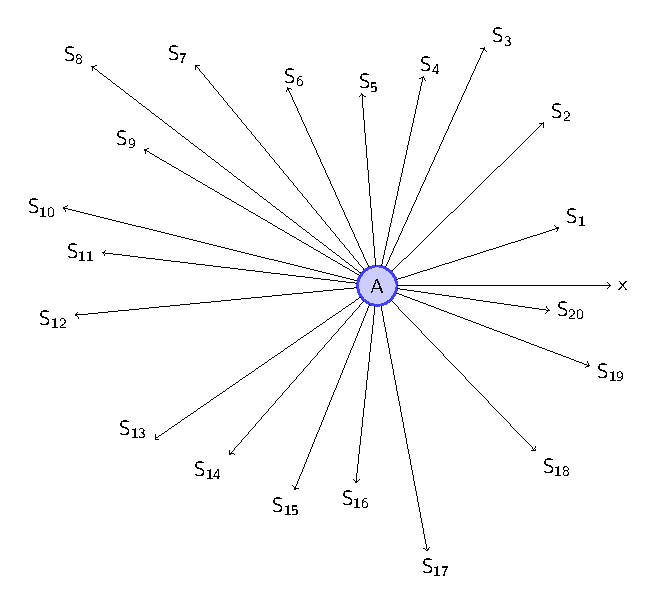
\includegraphics[scale=.5]{setSensors_1.pdf}
	\end{minipage}
	\hfill
	\begin{minipage}{.3\linewidth}
		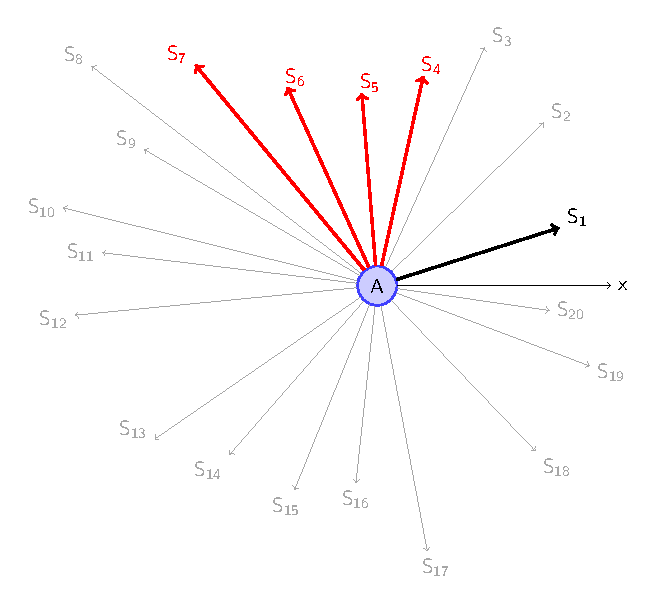
\includegraphics[scale=.5]{setSensors_2.pdf}
	\end{minipage}
	\hfill
	\begin{minipage}{.3\linewidth}
		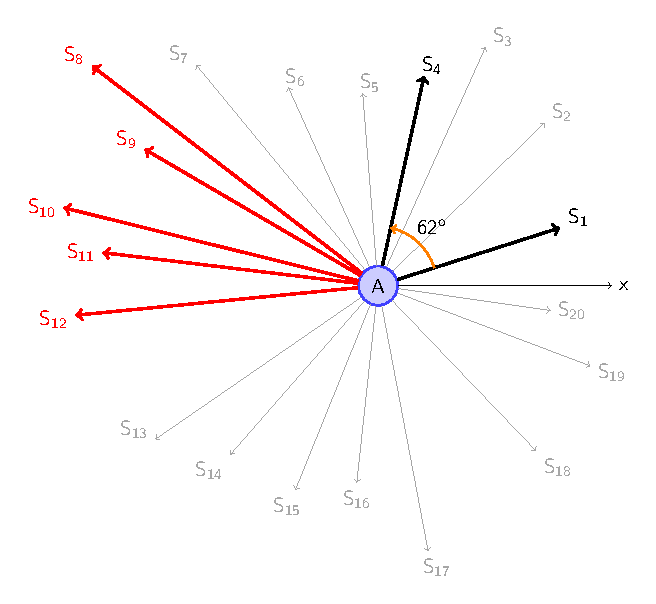
\includegraphics[scale=.5]{setSensors_3.pdf}
	\end{minipage}
	\\
	\begin{minipage}{.3\linewidth}
		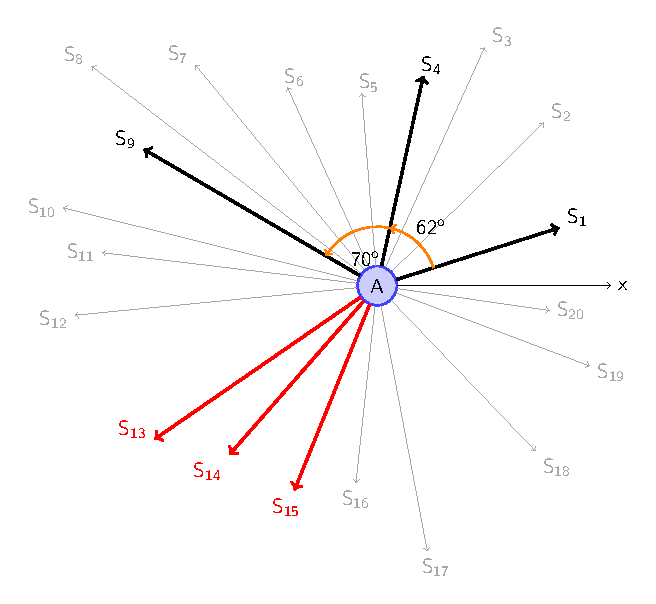
\includegraphics[scale=.5]{setSensors_4.pdf}
	\end{minipage}
	\hfill
	\begin{minipage}{.3\linewidth}
		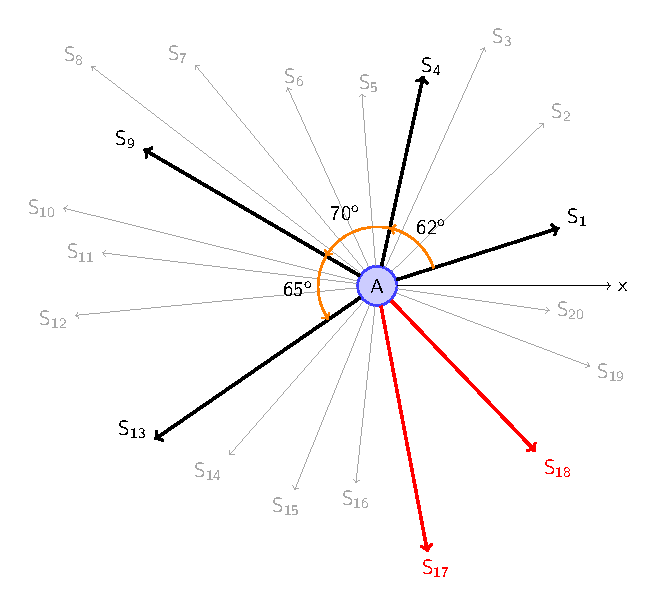
\includegraphics[scale=.5]{setSensors_5.pdf}
	\end{minipage}
	\hfill
	\begin{minipage}{.3\linewidth}
		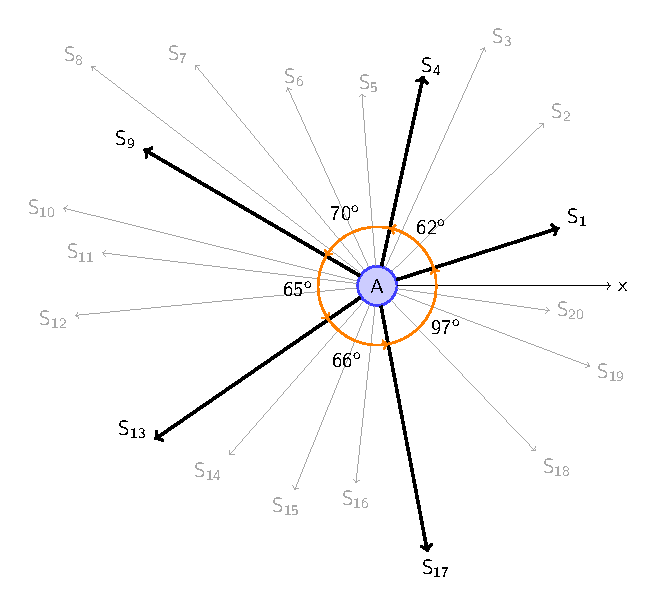
\includegraphics[scale=.5]{setSensors_6.pdf}
	\end{minipage}\\
	\caption{$L=\{S_1, S_4, S_9, S_{13}, S_{17}\}$ is a valid list with $k=5, \omega=60^o$}
	\label{finding}
\end{figure}

As aforementioned, when considering a sensor in $G$, it must satisfies some conditions to become candidate to be put into the list $L$. Suppose that at some point of the finding process, the list has {\sf\itshape index} elements and {\sf\itshape $L$[index] = $G$[current]}, {\sf\itshape 1} $\leq$ {\sf\itshape current} $\leq$ {\sf\itshape $n$}, $n$ is size of $G$. If {\sf\itshape $G$[next]} is chosen to be the next element in $L$, it must satisfy two conditions:
\begin{itemize}
	\item $(\overrightarrow{\vphantom{\overrightarrow{P}}PG\textsf{[cur]}}, \overrightarrow{\vphantom{\overrightarrow{P}}PG\textsf{[next]}}) > \omega \qquad (i)$
	\item $(\overrightarrow{\vphantom{\overrightarrow{P}}PG\textsf{[next]}}, \overrightarrow{\vphantom{\overrightarrow{P}}PL\textsf{[1]}}) > (k-\textsf{index})\omega \qquad (ii)$
\end{itemize}
From definition of ($k,\omega$) coverage, condition (i) is clearly necessary. However, it's not sufficient for {\sf\itshape $G$[next]} to become a candidate for the next position in $L$. If $L$ is a valid list, we have $(\overrightarrow{\vphantom{\overrightarrow{P}}PL[i]}, \overrightarrow{\vphantom{\overrightarrow{P}}PL[i+1]}) > \omega, i = \overline{1,k}$ (consider $k + 1 = 1$). Hence, $(\overrightarrow{\vphantom{\overrightarrow{P}}PL\textsf{[index + 1]}}, \overrightarrow{\vphantom{\overrightarrow{P}}PL[1]}) = \displaystyle\sum\limits_{i=\textsf{\scriptsize index} + 1}^{k}(\overrightarrow{\vphantom{\overrightarrow{P}}PL[i]}, \overrightarrow{\vphantom{\overrightarrow{P}}PL[i+1]}) > (k-\textsf{index})\omega$.
Since we are choosing candidate for {\sf (index + 1)-th} element in $L$, {\sf $G$[next]} corresponds to {\sf $L$[index + 1]}. Thus, (ii) is also a necessary condition.\\[7pt]
Algorithm \ref{alg00} and \ref{alg01} show the details of our method. Algorithm \ref{alg01} is a support function for Algorithm \ref{alg00}. {\tt RecurFinding(cur)} is a recursive function that finds candidate for {\sf (index + 1)-th} position in $L$ knowing that there is a set {\sf cur} containing the chosen sensors, in which the last sensor has index {\sf last}. It considers elements in $G$ sequentially from {\sf (last + 1)-th} element and checks if these elements satisfy condition (i) and (ii). The return value of {\tt RecurFinding(cur)} is a set containing all the lists of sensors that ($k-\omega$) cover the point $P$ which takes the current sublist ($\{L\textsf{[1]}, L\textsf{[1]},..., L\textsf{[index]}\}$) as its first {\sf index} elements exists. This return value is used to support the recursion process of the algorithm.

\noindent\begin{minipage}{.49\linewidth}
	\begin{algorithm}[H]
		\DontPrintSemicolon 
		\SetAlgoLined
		\newcommand{\forcondi}[2]{\ensuremath{#1 \in #2}}
		\SetKwData{found}{found}
		\SetKwData{Gsize}{G.size}
		\SetKw{true}{true}
		\SetKw{false}{false}
		\SetKwData{and}{\&\&}
		\SetKwData{equal}{==}
		\SetKwData{greater}{$\geq$}
		\SetKwData{notFound}{!found}
		\SetKwData{k}{k}
		\SetKwData{n}{n}
		\newcommand{\forcond}[3]{\ensuremath{#1 = #2\ \KwTo\ #3}}
		\BlankLine
		\KwIn{
			A point {\sf P} and a set {\sf G} consisting of {\sf n} sensors that cover {\sf P}.
		}
		\KwOut{
			\k sensors that ($\mathsf{k-\omega}$) covers {\sf P}. There is possibility that no output is found.
		}
		\BlankLine
		\BlankLine
		Let {\sf L} store the output\;
		Sort {\sf G} in counter-clockwise order around {\sf P}\;
		$L \leftarrow \emptyset$\;
		\For{\forcond{i}{1}{n}}{
			$temp \leftarrow {\tt RecurFinding(G{i})}$\;
			$L \leftarrow L \cup temp$\;
		}
		\caption{Find all lists of $k$ sensors that ({\sf $k-\omega$}) covers point $P$}
		\label{alg00}
	\end{algorithm}
\end{minipage}
\hfill
\begin{minipage}{.49\linewidth}
	\begin{algorithm}[H]
		\DontPrintSemicolon
		%	\SetAlgoNoLine
		%	\SetAlgoNoEnd
		\newcommand{\forcondi}[2]{\ensuremath{#1 \in #2}}
		\SetKwData{found}{found}
		\SetKwData{Gsize}{G.size}
		\SetKw{true}{true}
		\SetKw{false}{false}
		\SetKwData{and}{\&\&}
		\SetKwData{equal}{==}
		\SetKwData{greater}{$\geq$}
		\SetKwData{notFound}{!found}
		\SetKwData{k}{k}
		\SetKwData{n}{n}
		\SetKwData{cur}{cur}
		\SetKwArray{G}{G}
		\SetKwArray{L}{L}
		\SetKwData{P}{P}
		\SetKwFunction{Recur}{RecurFinding}
		\SetKwData{paratwo}{\tt index + 2, i}
		\SetKwData{paraone}{index + 1}
		\SetKwData{index}{index}
		\SetKw{return}{return}
		\SetKwProg{Fn}{}{}{end}
		\newcommand{\forcond}[3]{\ensuremath{#1 = #2\ \KwTo\ #3}}
		\BlankLine
		\KwIn{
			A list of sensors that is currently chosen, contains \index sensors.
		}
		\KwOut{
			All lists of \k sensors that ($k-\omega$) cover the point \sf P beginning with the input list.
		}
		\BlankLine
		\BlankLine
		\Fn{\tt RecurFinding({\sf cur})}{
			$L \leftarrow \emptyset$\;
			$\index \leftarrow$ cardinality of {\sf cur}\;
			\If{m \equal k}{\return {\sf \{cur\}}}
			$last \leftarrow$ index of last element in {\sf cur}\; 
			$first \leftarrow$ index of first element in {\sf cur}\;
			\For{\forcond{i}{last + 1}{\n}}{
				\If{
					$(\overrightarrow{\vphantom{\overrightarrow{P}} \P\G{last}}, \overrightarrow{\vphantom{\overrightarrow{P}} \P\G{i}}) > \omega$ \and
					$(\overrightarrow{\vphantom{\overrightarrow{P}} \P\G{i}}, \overrightarrow{\vphantom{\overrightarrow{P}} \P\G{first}}) > (\k - \index + 1)\omega$
				}{
					$temp \leftarrow$ {\tt RecurFinding({\sf cur} + (\G{i}))}\;
					$L \leftarrow L \cup temp$\;
				}
			}
			\return L\;
		}
		\caption{Find {\sf index + 1} element in {\sf L}}
		\label{alg01}
	\end{algorithm}
\end{minipage}

%\begin{figure*}[!h]
%\noindent\begin{minipage}{.49\linewidth}
%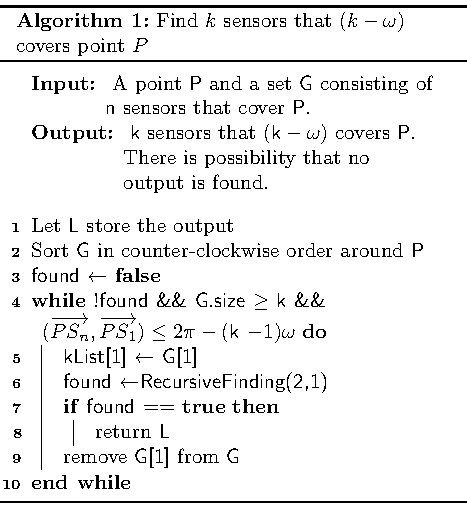
\includegraphics{Algo_1.pdf}
%\end{minipage}\hfill
%\begin{minipage}{.49\linewidth}
%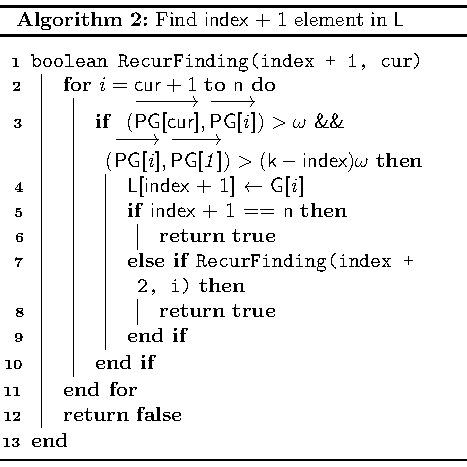
\includegraphics{Algo_2.pdf}
%\end{minipage}
%\end{figure*}

The first element of $L$ can be any sensor in $G$ since it doesn't require any condition. For convenient, we choose $L[1]=G[1]$. Thus, {\tt RecurFinding(\{G[1]\})} is called to start the finding process. After function call {\tt RecurFinding(\{G[1]\})}, the function will return all the satisfied lists containing G[1]. The finding process stops when we have called {\tt RecurFinding(\{G[$i$]\})} with every $i$ from 1 to n. And the algorithm will output a set containing all the lists of sensors that ($k-\omega$) cover the considered point $P$.

\subsubsection{Finding a barrier in a monitoring region}


a, Partitioning the monitoring region by Dynamic Partition method

\label{subsection1}

To find a barrier in the monitoring region, we first determine the areas that are multiple-view covered inside the region of interest $\Omega$. To solve this problem, we partition $\Omega$ into multiple small rectangles and check whether these rectangles are multiple-view covered or not. However, uniform partitioning often requires a high computation time especially when the $\Omega$ is large. To overcome this challenge, we propose a new partition method called Dynamic Partition. The idea of the Dynamic Partition method is as follows: only the rectangles which are not multiple-view covered will be partitioned into smaller rectangles, otherwise, they are kept untouched. \par
The first rectangle to be checked is the monitoring region. 
Using the algorithm in \ref{subsec:01}, if a rectangle is multiple-view covered, mark it as true, otherwise, split it into four equal sub-rectangles. After a rectangle is split, smaller rectangles are generated and the process of checking and splitting is applied to these new rectangles. A rectangle will not be split if it is multiple-view covered or its size reaches a predefined limited value. The smaller the limited size is, the more precise the result of our algorithm can get. This condition guarantees our algorithm not to go into an infinite loop. The process is illustrated in Figure \ref{dynamic}.
%\input{DynamicPartition}
\begin{figure}[h]
	\begin{center}
		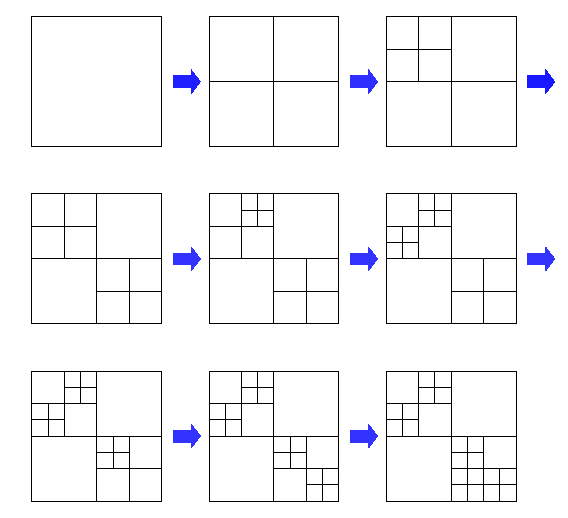
\includegraphics[scale=1.]{Dynamic_Partition.pdf}
	\end{center}
	\caption{Illustration of Dynamic Partitioning}
	\label{dynamic}
\end{figure}

The pseudo code of the method is described in Algorithm \ref{alg3}
%

%
\begin{center}
	\begin{minipage}{.7\linewidth}
		\begin{algorithm}[H]
			\DontPrintSemicolon
			\SetAlgoLined
			\newcommand{\forcondi}[2]{\ensuremath{#1 \in #2}}
			\SetKwData{Rcen}{root.center}
			\SetKwData{root}{rootRec}
			\SetKwData{RX}{root.sizeX}\SetKwData{RY}{root.sizeY}
			\SetKwData{L}{L}\SetKwData{W}{W}
			\SetKwData{QUEUE}{Q}
			\SetKwData{tempNode}{tempRec}
			\SetKwData{coveredGroup}{coveredGroup}
			\SetKwFunction{FAC}{findAndCheck}
			\SetKwData{coveredNodes}{coveredRectangles}
			\SetKwData{DMAX}{DMAX}
			\SetKwFunction{split}{split()}
			\SetKwFunction{makeNode}{makeNode}
			\SetKwFunction{dequeue}{dequeue}
			\SetKwFunction{enqueue}{enqueue}
			\SetKwFunction{check}{check}
			\SetKwData{tnRank}{tempRec.rank}
			\SetKwData{element}{element}
			\BlankLine
			\KwIn{
				\begin{itemize}
					\item \L, \W: Length and width of the monitoring region $\Omega$ respectively
					\item A set of deployed sensors $S$
					\item Minimum size of a grid
				\end{itemize}
			}
			\KwOut{A set of multiple-view covered rectangles $\Pi$}
			\BlankLine
			\BlankLine
%			Let \coveredNodes store the output\;
			Let \root denote the monitoring region\;
			$\QUEUE\gets$ \O \;
			\enqueue{\root, \QUEUE} \;
			\While{$\QUEUE \neq$ \O}{
				$\tempNode\gets$ \dequeue{\QUEUE}\;
%				Check if \tempNode is $(k-\omega)$ covered\;
				\uIf{\tempNode is multiple-view covered}{add \tempNode to $\Pi$\;}
				\ElseIf{\tempNode has not reached the minimum size}{split \tempNode into 4 sub-rectangles\;
					add 4 sub-rectangles of \tempNode to \QUEUE}
			}
			\caption{Dynamic Partition}
			\label{alg3}
		\end{algorithm}
	\end{minipage}
\end{center}

b, Finding a multiple-view coverage barrier

After procedure in \ref{subsec:01}, we now have a set $\Pi$ of rectangles that are multiple-view covered. To find a multiple-view covered barrier, we need to find a continuous area formed from rectangles in $\Pi$ that connects the left side to the right side of $\Omega$. The method is to transform the rectangles set into a graph. Each vertex in the graph corresponds to a rectangle in $\Pi$. Two vertices are considered adjacent if the corresponding rectangles share at least one point. Two virtual vertices are added to the graph, source vertex {\tt source} and sink vertex {\tt sink}. All vertices corresponding to the rectangles lying on the left side of $\Omega$ are adjacent to {\tt source} and all vertices corresponding to the rectangles lying on the right side of $\Omega$ are adjacent to {\tt sink}. After constructing the graph, we use Breath First Search algorithm to find a path from {\tt source} to {\tt sink}. If a path is found, we conclude that there exists a multiple-view barrier in the monitoring region. Otherwise, the barrier does not exist.

\subsection{Evaluate the quality of a ($k-\omega$) barrier}
\label{baCal}
The algorithm takes the nodes forming a barrier and the $k$-list of sensors associating with each node as the input and compute the coverage on the input barrier.

The coverage of the barrier is calculated as the average of every node which forms that barrier with the weight assigned as the area of each node. With $B_i$ as the nodes forming the barrier $B$, we have

$$E(B) = \iint_{B}E(P)dxdy.\frac{1}{S_B}$$

$$= (\sum_i(\iint_{B_i}E(P)dxdy)).\frac{1}{S_B}$$

$$=(\sum_iE(B_i).S_{B_i}).\frac{1}{S_B} $$

$$=(\sum_iE(B_i).S_{B_i}).\frac{1}{\sum_iS_{B_i}}$$

As a result, this calculation method is consistent with our definition of coverage on the barrier in the \ref{barrier} section, hence may provide preferable assessment on each setting of parameters.

Since it is impossible and unnecessary to compute the exact coverage value of each note, it is sufficient to publish a method to estimate an approximation of the coverage on the considered node. Take into account the fact that in each node is ($k-\omega$) covered by an unique $k$-list of sensors, hence the coverage value inside the node is a continuous function. As a result, we can create a dense grid in each node, and estimate the node coverage with the average of the vertices on the discrete grid. For convenience, the size of the grid is fixed to be the size of the node which will not be split further in \ref{subsection1}.

\section{Experimental results}

\subsection{Simulation method}

This part will analyze the effect of several parameters on 3 aspects of the result, which is the probability of creating barrier, the average coverage value of the multiple view sensor barrier and the overall computational time. The algorithm is performed on every instance and keep recording 3 metrics, the creation of barrier, the computational time and the coverage value on a barrier if there is one. Then, the result are combined for all instances of the same parameter settings to achieve the probability of barrier creation, the average computational time and the average coverage value corresponding to the setting of parameters.

\subsection{System setting and parameters setting}
%Đoạn này hư cấu sửa sau :v
System settings

All the experiments are performed on a personal computer with core Intel Core i7-7700HQ, 8GB of DDR4 RAM running on Windows 10 Home, the programming language used to simulate the algorithm is Java 11.

Parameter settings

The sensing fields in all experiments are presented as rectangles with the size of 200m x 50m. Sensor nodes are deployed uniformly in a rectangle with each side extended compared to the sides of the sensing field a distance equal to the sensing radius of each sensor in order to guarantee the uniform distribution regarding sensing area inside the sensing field. Each set of parameters contains several independent random topologies to conduct the algorithm on and measure the target indexes. The detailed reason for different settings of $k-\omega$ will be explained later in this section. Furthermore, each instance of experiment is conducted with both node handling methods. Altogether there are 42000 experiments on 210 instances of parameters which were analyzed with our algorithm. The details are as follows:
\begin{table}[h!]
	\centering
	\begin{tabular}{ll}
		\specialrule{1.pt}{0.pt}{1.pt}
		\specialrule{1.pt}{0.pt}{1.pt}
		\textbf{Parameters} & \textbf{Value} \\ \hline
		Length & 200 \\
		Width & 50 \\
		Sensing Radius & 30 \\
		Minimum sensing radius & 5 \\
		Sensing angle & 90 \\
		$k$ & 3, 4, 5, 6 \\
		The number of topologies for each instance & 100 \\
		Node handling method & Max, Random \\
		\specialrule{1.pt}{1.pt}{1.pt}
		\specialrule{1.pt}{0.pt}{1.pt}
	\end{tabular}
	\caption{General parameters}
\end{table}

\renewcommand{\arraystretch}{2}
\begin{table}[h!]
	\centering
	\begin{tabular}{|l | c | c | c | c|}
		\hline
		k & 3 & 4 & 5 & 6\\ \hline
		$\omega$ & 90 - 115 & 55 - 80 & 40 - 60 & 35 - 50\\ \hline
	\end{tabular}
	\caption{The value of $\omega$ correspond to each value of $k$}
\end{table}

\subsection{Computation results}

\subsubsection{Effect of $\omega$ on algorithm performance}

The parameter $\omega$ is an important factor in the multiple view coverage model. As a result, this parameter has a considerable impact on the output of the algorithm. Apparently it is meaningless to if value of $\omega$ greater or equal to $\frac{2\pi}{k}$, as it is impossible to achieve any $(k-\omega)$ cover at that settings. As a result, the analyzed values of $\omega$ are taken from around the upper bounds and decrease slowly for each value of $k$. To illustrate the result, Figure \ref{fig:wv}, \ref{fig:wt} and \ref{fig:wp} illustrate the effect of different values of $\omega$ on the outputs of the algorithm with 2 values of $k$ at the sensor number of 600.

Because $\omega$ is a lower bound for the angle between two consecutive sensors in the perspective of the considered point, every sensor set that satisfies the condition with large $\omega$ would also successfully make a $k-\omega$ cover with lower $\omega$. In short, a decrease in parameter $\omega$ may result in an expansion in the result space of the algorithm. This leads to two different consequences. On the one hand, there would be more sets of sensor $k-\omega$ cover a single node, which means that the coverage value of that node is likely to be lifted. However, on the other hand, the lower value of $\omega$ could reduce the average rank of the covered nodes, as the nodes are more easily covered, which leads to a lower coverage value, since the sets that cover the bigger node tend to position further than the sets covering the smaller ones.

As a consequence, firstly, with a lower value of $\omega$, the algorithm would offer a greater chance of $(k-\omega)$ barrier existence. However, the probability of forming barriers can never exceed $100\%$, the curve that represents the barrier probability would approach $100\%$ and does not rise higher with lower $\omega$. Regarding coverage value, while the max method illustrate an downward trend, the random method tends to go up while the value of $\omega$ keep rising. This result is not applied to very large value of $\omega$, where the low barrier probability leads to little number of examined sensing field, which results in a high variance and the obtained results would be less concrete. However, despite overall trends, the coverage value obtained with different $\omega$ is observed not to change significantly, and the difference can be accepted in real circumstances.

Finally, a lower value of $\omega$ results in a larger searching space, which leads to a drastic rise in computation time to conduct the max method, while the random method does not suffer from this property. This result may come from the fact that the max method require the evaluation of the coverage value of every $(k-\omega)$ sensor list toward each node, which seems to be an exception job.

\begin{figure}[!h]
	\begin{subfigure}[t]{.5\textwidth}
		\centering
		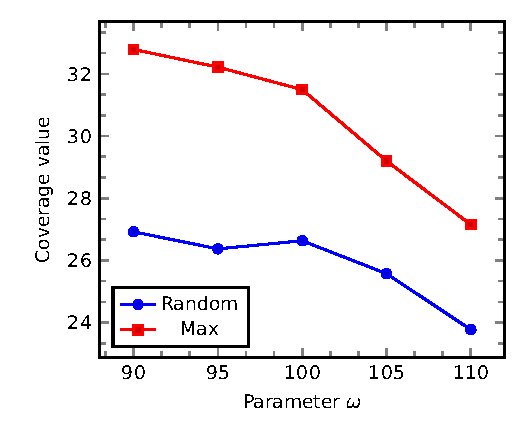
\includegraphics[scale=.8]{Hinhanh/OmegaEffect/coverage/k3.pdf}
		\caption{k = 3}
	\end{subfigure}
%	\hfill
	\begin{subfigure}[t]{.5\textwidth}
		\centering
		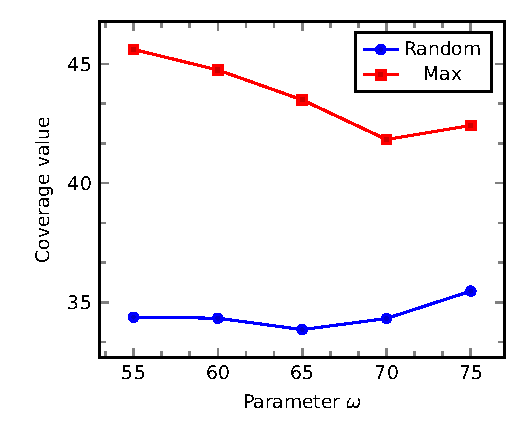
\includegraphics[scale=.8]{Hinhanh/OmegaEffect/coverage/k4.pdf}		
		\caption{k = 4}
	\end{subfigure}
\caption{Effect of $\omega$ on the average coverage value of the found barrier with $k = 3$ and $k = 4$}
\label{fig:wv}
\end{figure}
%
\begin{figure}[!h]
	\begin{subfigure}[t]{.5\textwidth}
		\centering
		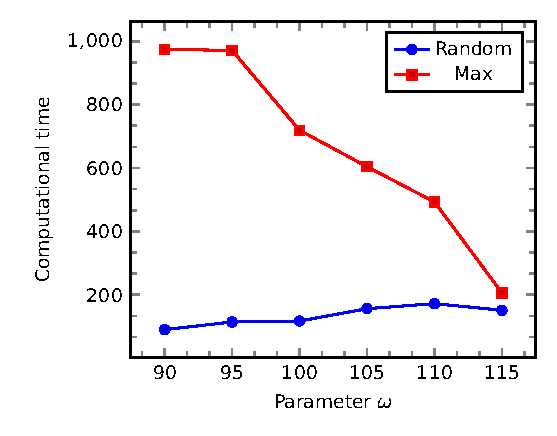
\includegraphics[scale=.8]{Hinhanh/OmegaEffect/time/k3.pdf}		
		\caption{k = 3}
	\end{subfigure}
	\begin{subfigure}[t]{.5\textwidth}
		\centering
		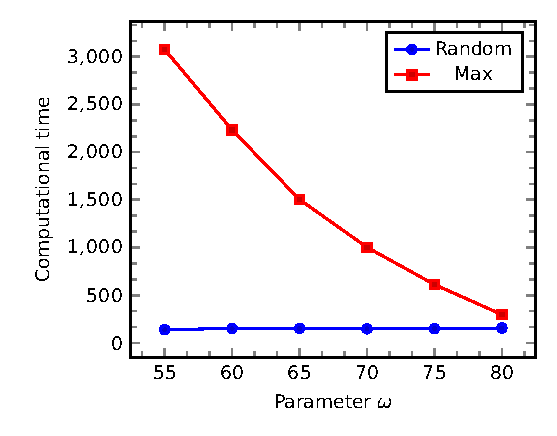
\includegraphics[scale=.8]{Hinhanh/OmegaEffect/time/k4.pdf}		
		\caption{k = 4}
	\end{subfigure}
\caption{Effect of $\omega$ on the average computational time in $ms$ of the algorithm with $k = 3$ and $k = 4$}
\label{fig:wt}
\end{figure}
%
\begin{figure}[!h]
	\begin{subfigure}[t]{.5\textwidth}
		\centering
		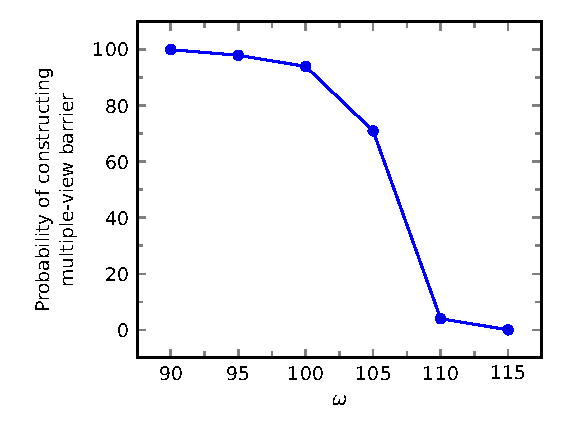
\includegraphics[scale=.8]{Hinhanh/OmegaEffect/probability/k3.pdf}		
		\caption{k = 3}
	\end{subfigure}
	\begin{subfigure}[t]{.5\textwidth}
		\centering
		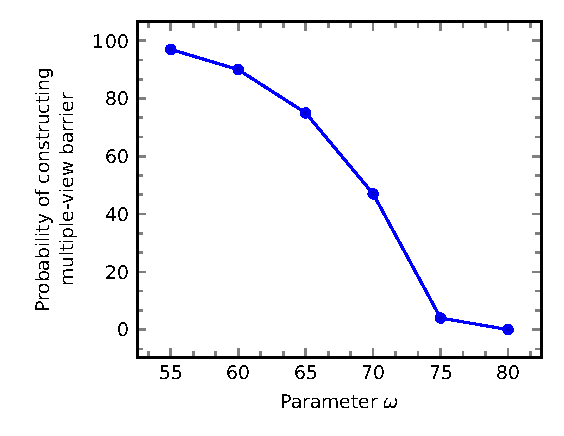
\includegraphics[scale=.8]{Hinhanh/OmegaEffect/probability/k4.pdf}		
		\caption{k = 4}
	\end{subfigure}
\caption{Effect of $\omega$ on the probability of existence of multiple view barrier with $k = 3$ and $k = 4$}
\label{fig:wp}
\end{figure}

\subsubsection{Effect of sensor number on algorithm performance}

Figure \ref{fig:nv}, \ref{fig:nt} and \ref{fig:np} illustrate the effect of different values of sensor number on the outputs of the algorithm with setting of parameters $k$, $\omega$. Similar to the effect of $\omega$, a larger value of sensor number would lead to a larger searching space. However, in this occasion, the negative effect on coverage value seems to be more significant. As a result, the barrier coverage value tends to fall slowly as the sensor number rises for both node handling methods. Furthermore, the large number of sensors leads to a huge computational work, as the time required to run both methods rise linearly with the increase of the sensor number. This results in the computation time surge dramatically as the sensor number grows.

\begin{figure}[!h]
	\begin{subfigure}{.5\textwidth}
		\centering
		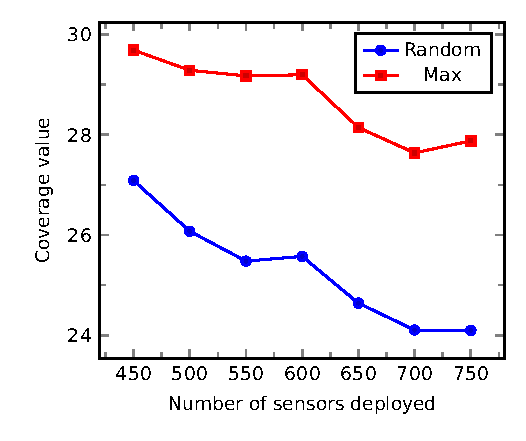
\includegraphics[scale=.8]{Hinhanh/SensorNumberEffect/coverage/k3omega105.pdf}
		\caption{k = 3, $\omega$ = 105}
	\end{subfigure}
	\begin{subfigure}{.5\textwidth}
		\centering
		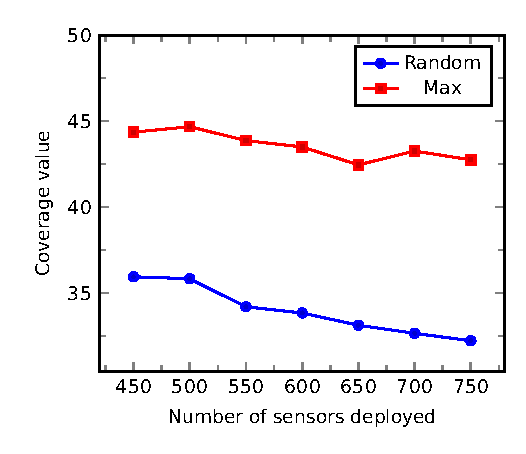
\includegraphics[scale=.8]{Hinhanh/SensorNumberEffect/coverage/k4omega65.pdf}
		\caption{k = 4, $\omega$ = 65}
	\end{subfigure}
\caption{Effect of sensor number on the average coverage value of the found barrier with some typical values of $k$ and $\omega$}
\label{fig:nv}
\end{figure}
%
\begin{figure}[!h]
	\begin{subfigure}{.5\textwidth}
		\centering
		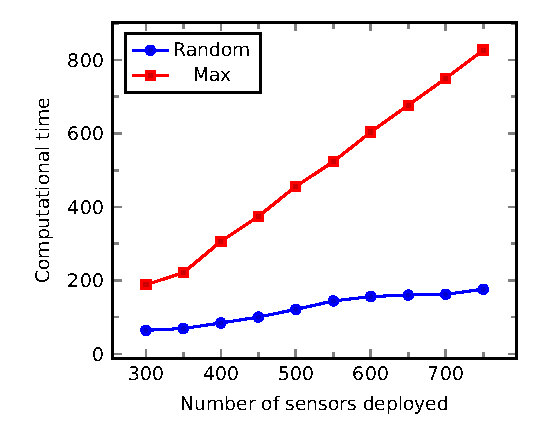
\includegraphics[scale=.8]{Hinhanh/SensorNumberEffect/time/k3omega105.pdf}
		\caption{k = 3, $\omega$ = 105}
	\end{subfigure}
	\begin{subfigure}{.5\textwidth}
		\centering
		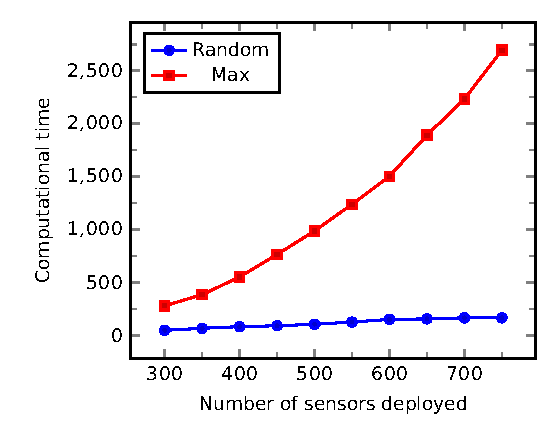
\includegraphics[scale=.8]{Hinhanh/SensorNumberEffect/time/k4omega65.pdf}
		\caption{k = 4, $\omega$ = 65}
	\end{subfigure}
\caption{Effect of sensor number on the average computational time in $ms$ of the algorithm with some typical values of $k$ and $\omega$}
\label{fig:nt}
\end{figure}
%
\begin{figure}[!h]
	\begin{subfigure}{.5\textwidth}
		\centering
		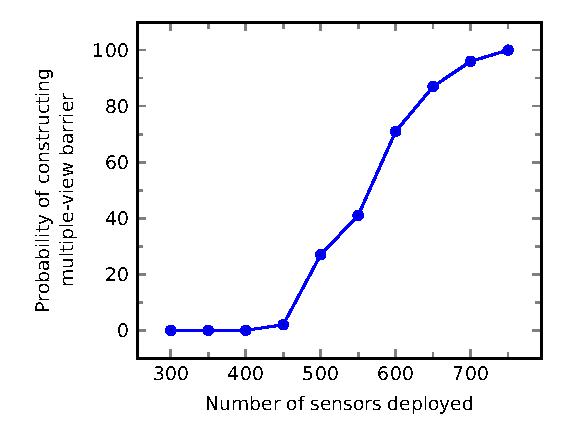
\includegraphics[scale=.8]{Hinhanh/SensorNumberEffect/probability/k3omega105.pdf}
		\caption{k = 3, $\omega$ = 105}
	\end{subfigure}
	\begin{subfigure}{.5\textwidth}
		\centering
		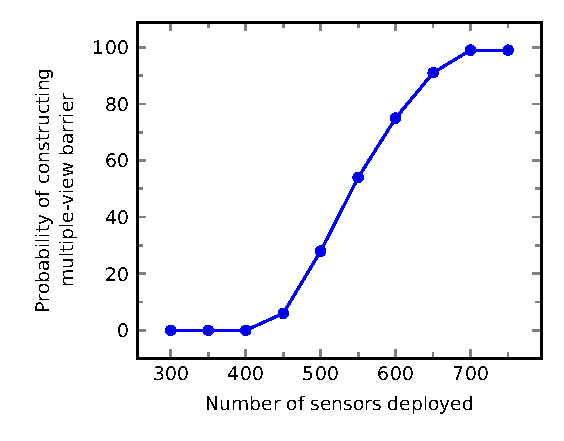
\includegraphics[scale=.8]{Hinhanh/SensorNumberEffect/probability/k4omega65.pdf}
		\caption{k = 4, $\omega$ = 65}
	\end{subfigure}
\caption{Effect of sensor number on the probability of existence of multiple view barrier with some typical values of $k$ and $\omega$}
\label{fig:np}
\end{figure}

\subsubsection{Effect of $k$ on algorithm performance}

The parameter $k$ is affected the achieved results the most regarding all 3 aspects. This is because the change in $k$ would manipulate the problem entirely, an answer with a value of $k$ would not be an answer with another value of $k$. As a consequence, the achieved results are drastically different among every value of $k$.

As mentioned in previous parts, generally, the coverage value of the barriers would not be much different from the others. As a result, we may reach a conclusion that for every value of $k$, it is possible to define a critical value of barrier coverage which denotes the largest achieved value of coverage for a certain value of $k$. And this critical coverage value could be use to compare the performance of the problem with different values of $k$.

Regarding this metric, in general, as there are more sensors that cover a certain point, an increase in the value of $k$ may lead to a larger critical coverage value. However, since the function of $cos(x)$ has a derivative getting lower as the value of $x$ comes close to 0, and the effect of increasing $k$ on decreasing the sight angle of sensors to the parts of the intruder ($\phi - \phi_i$) may reduce with larger $k$. As a result, the critical coverage value would rise slower than the rise in the value of $k$.

Finally, the effect of $k$ on computation time is hard to illustrate clearly, since each $k$ would correspond to different values of $\omega$, which makes it impossible to choose which settings of parameters should be compared. However, in general, a greater amount of $k$ would lead to a significant greater computational time. This is because that the large value of $k$ would leads to a larger nest in traversing for all the $k-\omega$ sets and larger loop when checking the coverage value of nodes, hence the computation time for finding all the sets that $k-\omega$ cover each node and determining the sets of sensor with largest coverage value is increased considerably.

Consequently, it is appropriate to conduct the algorithm with some values of $k$ that is not too small, as the coverage value would be too low and not too large, as the coverage value would not be improve significantly compared to the previous value, the computational time would be exceptional and also the number of sensors in each cover would be unnecessary.

\begin{figure}[!h]
	\centering
	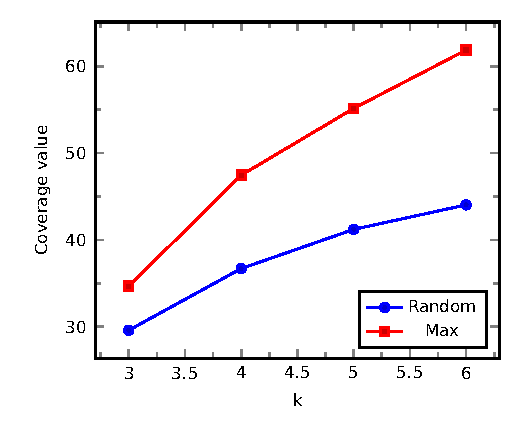
\includegraphics[scale=1.]{Hinhanh/kEffect/main.pdf}
	\caption{Effect of $k$ on the critical coverage value of the $(k-\omega)$ barrier}
	\label{fig:k}
\end{figure}

\subsection{Experimental conclusion}
Regarding all above analysis, it is possible to achieve some valuable conclusion about the model of $(k-\omega)$.
\begin{itemize}
	\item Firstly, it is notable that the max method overcomes the random method regarding coverage value with a considerable gap between the method results. Despite the surge in computational time due to expensive node handling, the significant offered coverage value prove that it is more suitable to choose the max node handling method.
	\item In terms of model parameters $k$, $\omega$ and sensor number, with the choose of max method, the model offer great result regarding coverage value, computational time and barrier probability with some appropriate settings of parameters.
\end{itemize}

\section{Conclusion}
%
This paper addressed the minimal exposure path problem for attenuated sensing model with all mobile sensors. We first have considered and formulated a model of the minimal exposure path problem in all mobile sensor networks; we have proposed the genetic algorithm to solve this issue. In addition, extensive experimental simulations were conducted to validate and to evaluate the proposed model as well as algorithm. The results showed that: the proposed algorithm could be effectively applied to both static and mobile models of wireless sensor networks; the coverage of mobile sensor networks is almost better than the coverage of static sensor networks in case having the same number of sensors.

%\bibliography{mybibfile}
\bibliography{report}
\bibliography{mybibfile}
\end{document}